
Dựa trên các nghiên cứu lý thuyết ở chương trước, chương này trình bày
kiến trúc thực tế đã được hiện thực hóa cho hệ thống Trục tích hợp dữ
liệu. Kiến trúc được điều chỉnh so với đề xuất ban đầu để phù hợp với
phạm vi dự án capstone và các ràng buộc kỹ thuật thực tế.

\section{Thiết kế kiến trúc}

\subsection{Yêu Cầu Chức Năng và Phi Chức Năng}

\textbf{Yêu Cầu Chức Năng}

\begin{itemize}
    \item \textbf{Tích hợp dữ liệu từ hệ thống nguồn:} Hệ thống kết nối
    và trích xuất dữ liệu từ API của hệ thống nguồn thông qua giao thức
    HTTP/REST, hỗ trợ phân trang và xử lý dữ liệu theo lô.

    \item \textbf{Đồng bộ theo nhiều chiến lược:} Hỗ trợ ba chiến lược
    đồng bộ — \texttt{upsert} (thêm mới hoặc cập nhật), \texttt{incremental}
    (chỉ xử lý bản ghi thay đổi theo \texttt{updatedAfter}), và
    \texttt{overwrite} (xóa toàn bộ rồi ghi lại) — được cấu hình riêng cho
    từng bảng thông qua Schema Registry.

    \item \textbf{Lập lịch đồng bộ tự động:} Cho phép tạo, cấu hình và
    kích hoạt/vô hiệu hóa các tác vụ đồng bộ định kỳ thông qua biểu thức
    cron. Lịch được lưu trong MongoDB và nạp động vào bộ lập lịch khi khởi
    động.

    \item \textbf{Quản lý schema:} Tự động phát hiện thay đổi cấu trúc dữ
    liệu tại hệ thống nguồn thông qua so sánh hash. Khi schema thay đổi,
    bảng bị khóa khỏi chu kỳ đồng bộ cho đến khi quản trị viên xem xét và
    phê duyệt.

    \item \textbf{Sao lưu và phục hồi:} Tự động tạo snapshot trước mỗi lần
    sync, sau mỗi thay đổi schema và theo lịch hàng tuần. Hỗ trợ restore
    về bất kỳ điểm nào trong lịch sử backup.

    \item \textbf{Xác thực và phân quyền:} Mọi yêu cầu API đều phải qua
    xác thực JWT. Phân quyền theo vai trò kết hợp phạm vi bảng dữ liệu
    cụ thể.

    \item \textbf{Giám sát và cảnh báo:} Thu thập metrics qua Prometheus,
    hiển thị trên Grafana, và gửi email cảnh báo khi tác vụ đồng bộ thất
    bại.
\end{itemize}

\textbf{Yêu Cầu Phi Chức Năng}

\begin{itemize}
    \item \textbf{Tính bảo mật:} Mật khẩu được băm bằng \texttt{bcrypt}.
    Token JWT ký bằng khóa bí mật. Toàn bộ giao tiếp qua Kong API Gateway
    với kiểm soát CORS và xác thực token tập trung.

    \item \textbf{Tính bền vững dữ liệu:} Backup đa lớp (MinIO nội bộ +
    AWS S3 đám mây) đảm bảo dữ liệu không bị mất ngay cả khi hạ tầng
    on-premise gặp sự cố.

    \item \textbf{Khả năng quan sát:} Toàn bộ sự kiện đồng bộ, lỗi và
    kết quả được ghi vào Event Log (MongoDB). Metrics được thu thập và
    hiển thị theo thời gian thực trên Grafana.

    \item \textbf{Khả năng bảo trì:} Backend được tổ chức theo mô hình
    module hóa của NestJS — mỗi module có trách nhiệm duy nhất, dễ dàng
    mở rộng hoặc thay thế độc lập.

    \item \textbf{Tính sẵn sàng:} Tất cả container được cấu hình
    \texttt{restart: always} — tự động khởi động lại sau sự cố hoặc khi
    máy chủ reboot.
\end{itemize}

\newpage
\subsection{Sơ Đồ Kiến Trúc Tổng Thể}

So với kiến trúc lý thuyết API-led Connectivity ba lớp (System API,
Process API, Experience API) ban đầu, kiến trúc thực tế được hợp nhất
thành một \textbf{backend monolith} theo mô hình module hóa của NestJS.
Quyết định này xuất phát từ phạm vi dự án capstone: số lượng nguồn dữ
liệu, lưu lượng và team size chưa đủ để hiện thực kiến trúc microservice đầy đủ.

\begin{figure}[!htp]
    \centering
    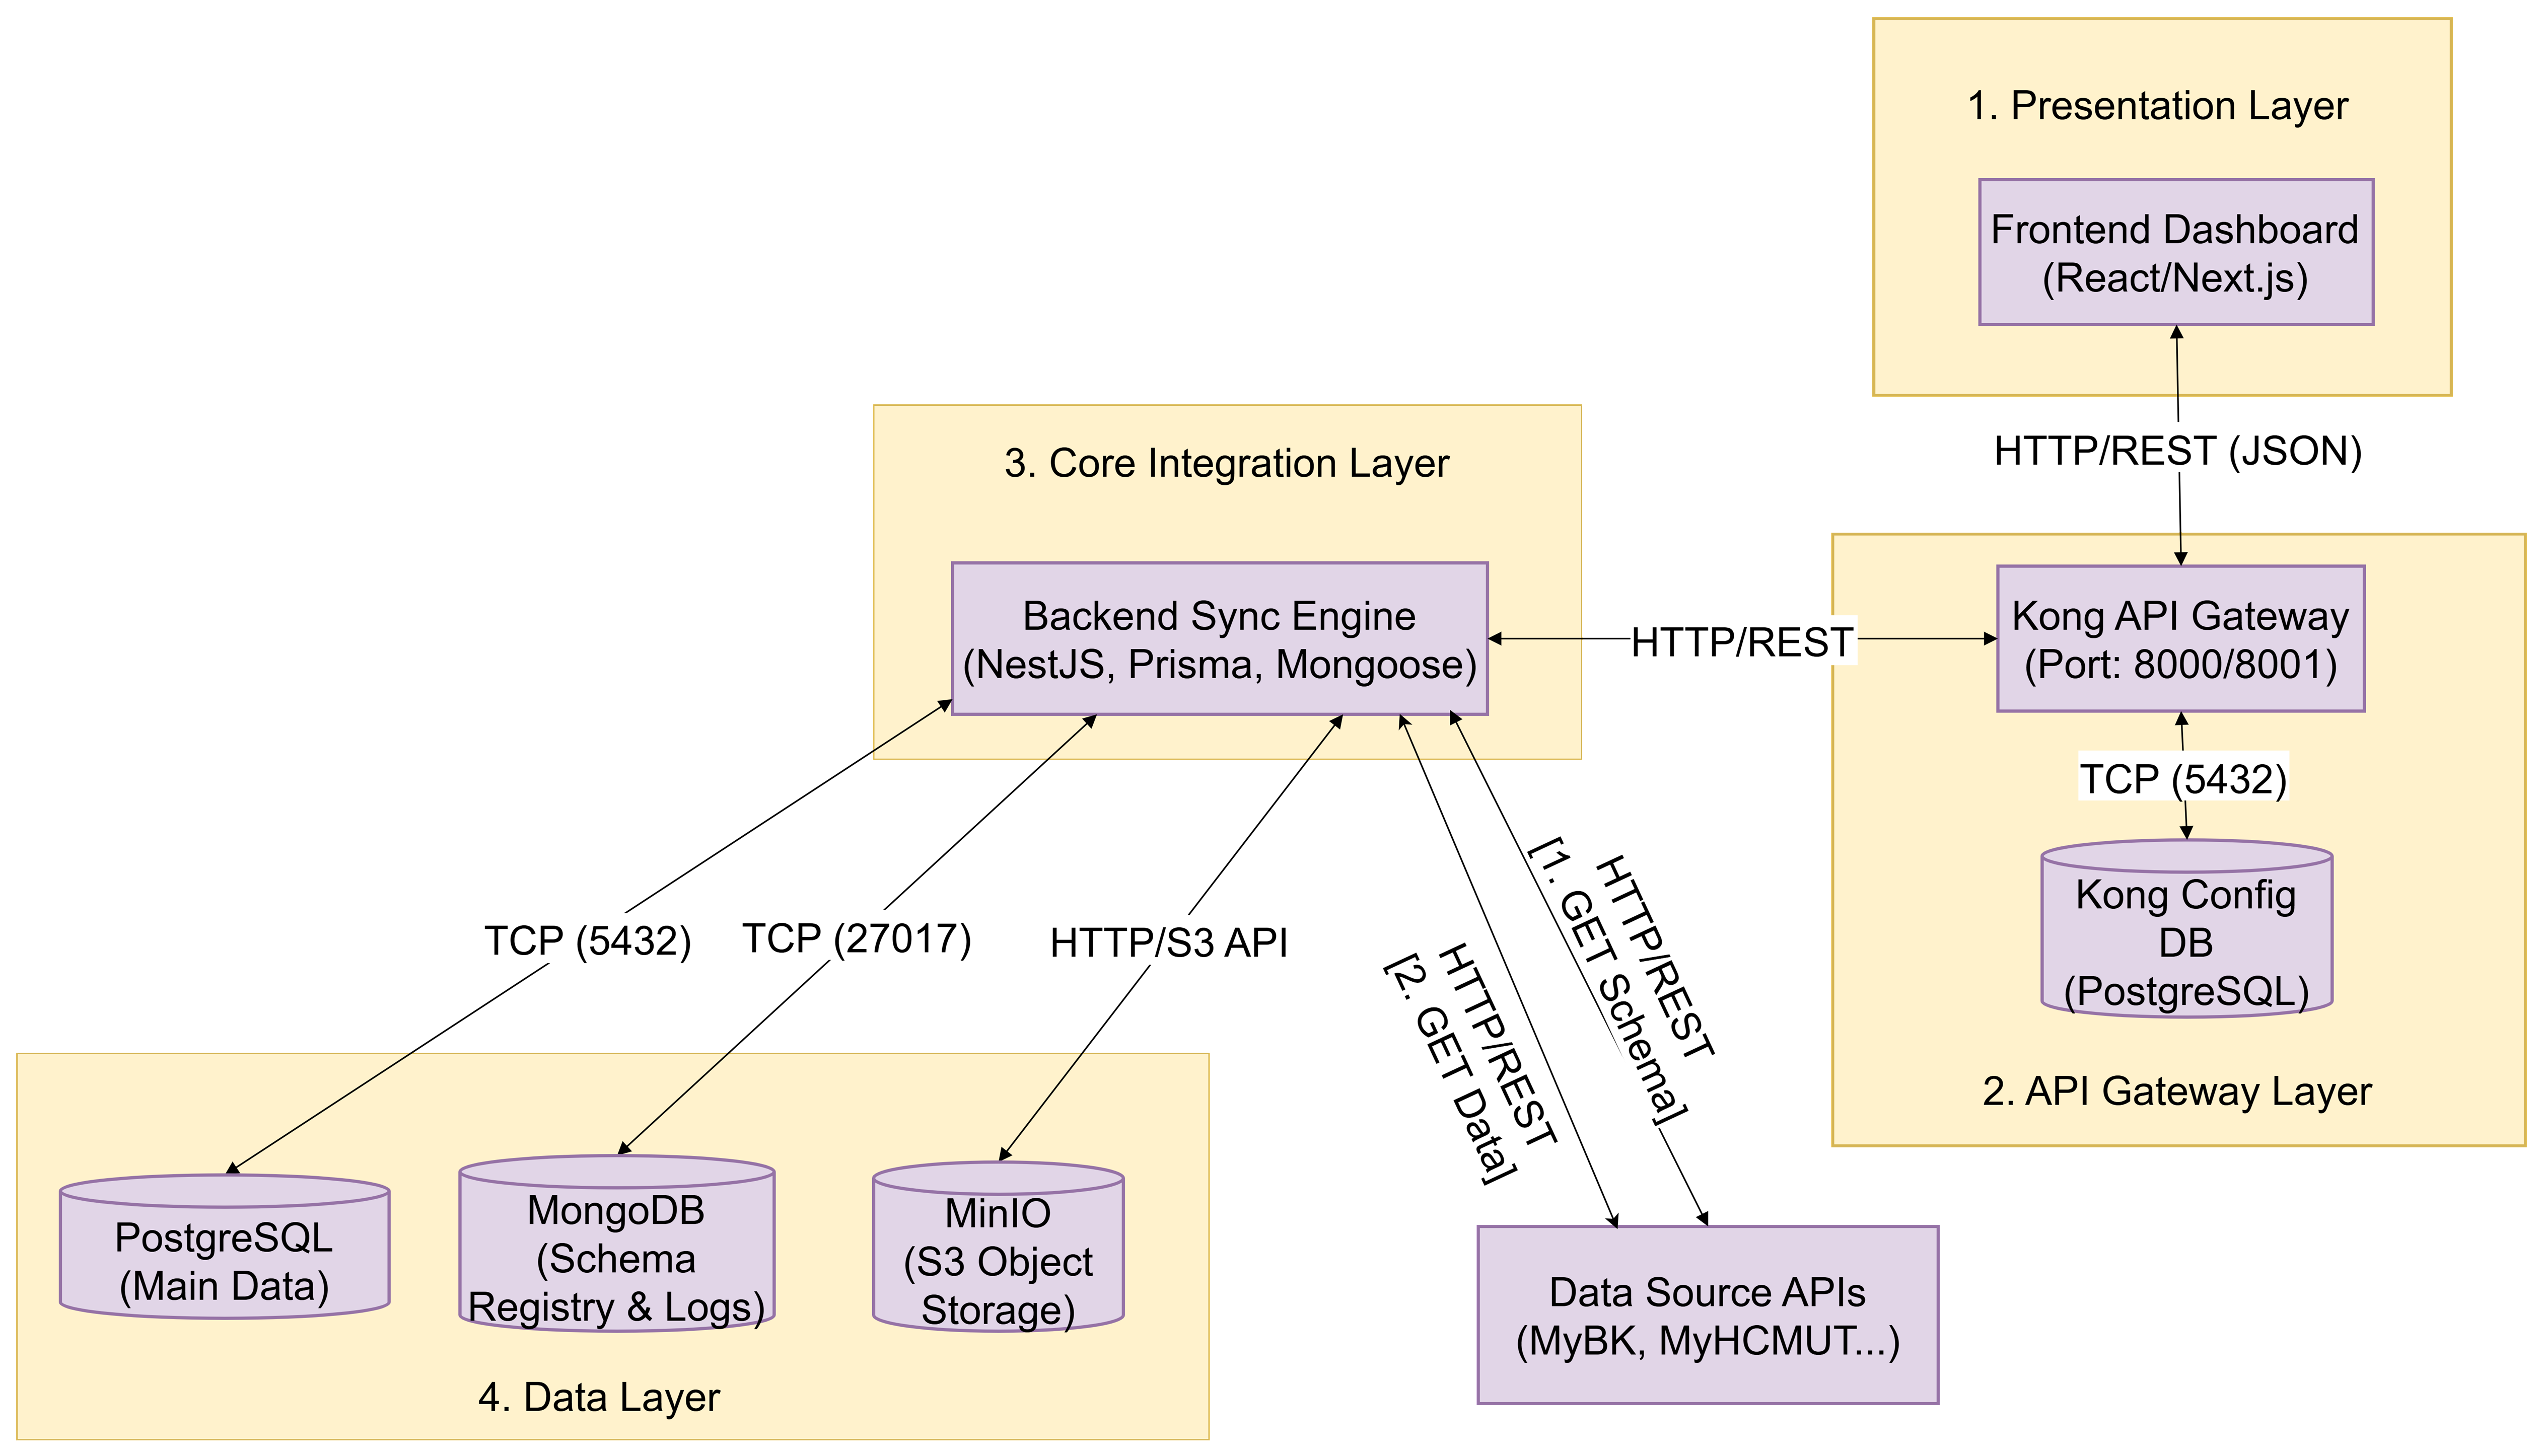
\includegraphics[width=0.9\textwidth]{graphics/overall.png}
    \caption{Sơ đồ kiến trúc tổng thể}
    \label{fig:refresh_token_flow}
\end{figure}

\newpage

\subsection{Giải Thích Chi Tiết Các Thành Phần}

\subsubsection{Admin Dashboard (Next.js Frontend)}

Giao diện quản trị được xây dựng bằng Next.js, đóng vai trò là điểm
tương tác duy nhất cho quản trị viên. Các chức năng chính bao gồm: quản
lý người dùng và phân quyền, theo dõi lịch sử đồng bộ qua Event Log,
kích hoạt và giám sát tác vụ đồng bộ, quản lý Schema Registry, và thao
tác với hệ thống backup.

Frontend giao tiếp hoàn toàn qua Kong API Gateway, không gọi trực tiếp
vào backend. Biến \texttt{NEXT\_PUBLIC\_KONG\_URL} được nhúng vào bundle
tại thời điểm build — thay đổi địa chỉ yêu cầu build lại container.

\subsubsection{Kong API Gateway}

Kong là cổng vào duy nhất cho mọi yêu cầu từ frontend. Cấu hình được
quản lý khai báo qua file \texttt{kong.yml} và đồng bộ vào Kong runtime
thông qua công cụ \texttt{deck}. Các trách nhiệm của Kong:

\begin{itemize}
    \item \textbf{Định tuyến:} Ánh xạ các đường dẫn
    (\texttt{/auth}, \texttt{/users}, \texttt{/integration}, v.v.) tới
    backend tại \texttt{http://backend:4000/api/v1}.
    \item \textbf{CORS:} Plugin CORS kiểm soát các origin được phép gọi
    API — quan trọng khi triển khai trên EC2 với Public IP cụ thể.
    \item \textbf{Metrics:} Plugin Prometheus thu thập số liệu về lưu
    lượng và độ trễ của từng route.
\end{itemize}

\subsubsection{NestJS Backend (Monolith)}

Backend là một ứng dụng NestJS duy nhất, được tổ chức thành các module
độc lập. Mỗi module đóng gói controller, service và các dependency của
riêng nó.

\paragraph{Auth Module và Users Module}

Hai module này hiện thực hóa cơ chế xác thực và phân quyền. Xác thực
dựa trên JWT với Passport.js. Phân quyền theo mô hình vai trò hai cấp:
vai trò cứng (\texttt{admin}, \texttt{reader}, \texttt{writer}) kết hợp
phạm vi bảng dữ liệu linh hoạt qua \texttt{roleSettings} dạng regex
pattern. Chi tiết được trình bày tại Chương~\ref{auth}.

\paragraph{Schema Registry Module}

Lưu trữ metadata của từng bảng dữ liệu trong MongoDB, bao gồm: chiến
lược đồng bộ (\texttt{syncStrategy}), khóa chính, danh sách trường, hash
của cấu trúc hiện tại, trạng thái (\texttt{stable} / \texttt{changed} /
\texttt{new}), và thời điểm đồng bộ gần nhất (\texttt{lastSyncTime}).

Mỗi lần pipeline chạy, Schema Registry so sánh hash cấu trúc trả về từ
API nguồn với hash đang lưu. Nếu phát hiện thay đổi, bảng bị đánh dấu
\texttt{changed}, emit event \texttt{schema.changed} để kích hoạt backup
kiểm toán, và bị loại khỏi chu kỳ sync cho đến khi admin xem xét.

\paragraph{Data Integration Module}

Đây là module trung tâm, hiện thực hóa toàn bộ pipeline ETL. Khi được
kích hoạt (thủ công hoặc qua lịch), module thực hiện tuần tự:

\begin{enumerate}
    \item Lấy danh sách bảng \texttt{stable} từ Schema Registry.
    \item Với mỗi bảng: tạo pre-sync backup, sau đó fetch dữ liệu từ API
    nguồn theo chiến lược đã cấu hình.
    \item Ghi dữ liệu vào PostgreSQL thông qua Sync Engine.
    \item Phát hiện orphan records (bản ghi tồn tại ở destination nhưng
    không còn ở source) nếu điều kiện cho phép.
    \item Ghi kết quả vào Event Log và gửi email thông báo qua
    Notification Module.
\end{enumerate}

Module hỗ trợ hai loại pipeline: \textbf{Full Sync} (toàn bộ bảng
stable) và \textbf{Custom Sync} (danh sách bảng do admin chỉ định).

\paragraph{Job Scheduler Module}

Quản lý các tác vụ đồng bộ định kỳ. Mỗi tác vụ được lưu trong MongoDB
với biểu thức cron, loại job (\texttt{FULL\_SYNC}), trạng thái
(\texttt{active}/\texttt{inactive}) và thời điểm chạy gần nhất.

Khi backend khởi động, toàn bộ tác vụ active được đăng ký động vào
\texttt{SchedulerRegistry} của NestJS. Admin có thể tạo, sửa,
bật/tắt và kích hoạt thủ công tác vụ qua API mà không cần restart
server.

\paragraph{Backup Module}

Quản lý toàn bộ vòng đời backup: tạo snapshot (4 trigger), liệt kê,
tải về, xóa và restore. Backup được lưu trên MinIO theo cấu trúc \newline
\texttt{\{trigger\}/\{tableName\}/\{timestamp\}.json}. Admin có thể
đồng bộ thủ công lên AWS S3 để lưu trữ vĩnh viễn. Chi tiết được trình
bày tại Chương~\ref{backup}.

\paragraph{Event Log Module}

Ghi nhận mọi sự kiện đáng chú ý vào MongoDB: bắt đầu/kết thúc pipeline,
thành công/thất bại của từng bảng, phát hiện orphan, restore backup.
Event Log là nguồn dữ liệu chính để admin theo dõi lịch sử hoạt động
của hệ thống.

\paragraph{Notification Module}

Gửi email cảnh báo qua SMTP (Gmail) khi tác vụ đồng bộ thất bại hoặc
hoàn thành. Email chứa thông tin: tên tác vụ, thời gian, thời lượng
thực thi, và chi tiết lỗi (nếu có). Module được đánh dấu \texttt{@Global}
để có thể inject vào bất kỳ module nào mà không cần khai báo lại.

\begin{figure}[!htp]
    \centering
    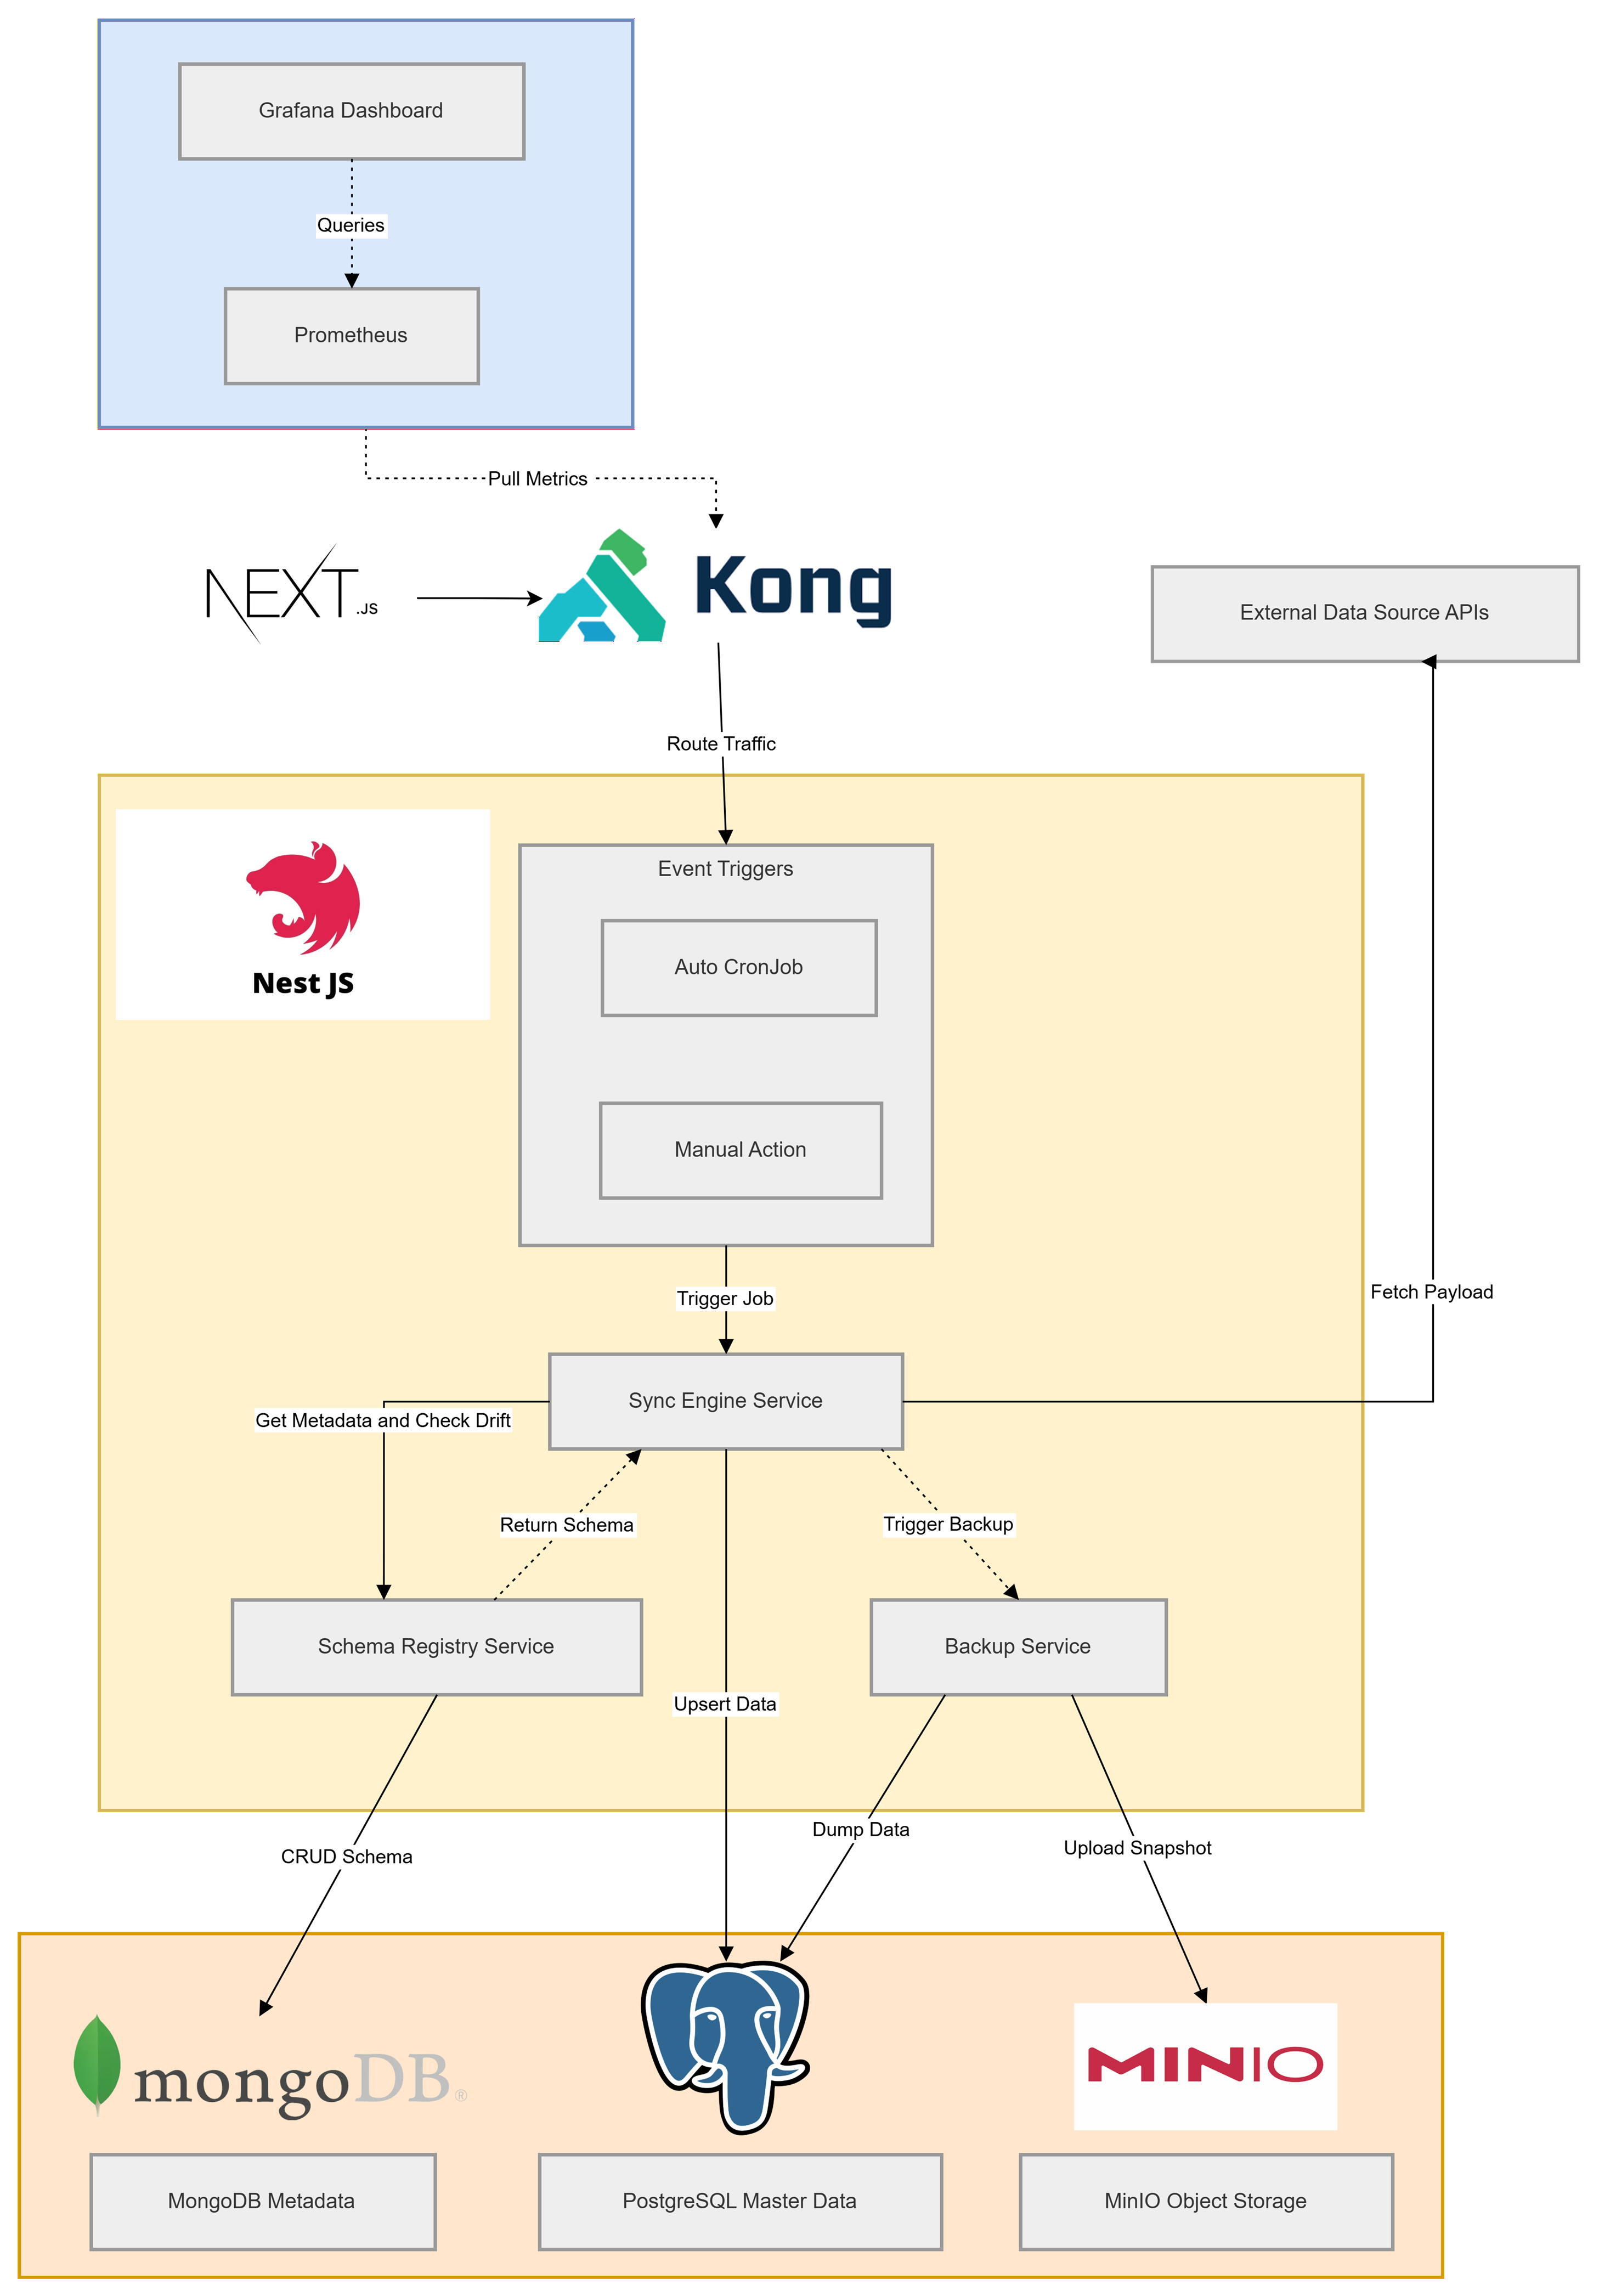
\includegraphics[width=0.9\textwidth]{graphics/detailed.png}
    \caption{Tương tác giữa các module backend và với các thành phần bên ngoài}
\end{figure}

\subsubsection{Tầng Lưu Trữ}

\paragraph{PostgreSQL (qua Prisma ORM)}

Cơ sở dữ liệu quan hệ chính, lưu trữ toàn bộ dữ liệu nghiệp vụ đã được
đồng bộ từ các hệ thống nguồn, cùng với thông tin người dùng và cấu hình
retention policy. Prisma ORM đảm bảo type-safety và quản lý migration có
kiểm soát.

\paragraph{MongoDB (qua Mongoose)}

Cơ sở dữ liệu document, lưu trữ ba loại dữ liệu vận hành:
Schema Registry (metadata và cấu hình đồng bộ của từng bảng), Event Log
(nhật ký hoạt động), và Scheduled Jobs (cấu hình tác vụ định kỳ). MongoDB
Atlas được sử dụng dưới dạng dịch vụ cloud — không cần triển khai và
quản lý MongoDB server.

\paragraph{MinIO và AWS S3}

Lưu trữ backup theo kiến trúc hai tầng: MinIO (self-hosted, độ trễ thấp)
và AWS S3 (cloud, lưu trữ vĩnh viễn). Chi tiết tại
Chương~\ref{backup}.

\subsubsection{Hệ Thống Nguồn Dữ Liệu}

Trong phạm vi dự án, hệ thống nguồn là một REST API cung cấp dữ liệu
sinh viên qua giao thức HTTP. API trả về dữ liệu theo định dạng chuẩn:

\begin{verbatim}
{
  "success": true,
  "metadata": { "totalRecords": 68411, "totalPages": 14 },
  "payload": [ { "id": 1, ... } ]
}
\end{verbatim}

Hệ thống tích hợp đóng vai trò consumer thuần túy — chỉ đọc dữ liệu qua
API, không kết nối trực tiếp vào cơ sở dữ liệu nguồn.

\subsubsection{Giám Sát: Prometheus và Grafana}

Prometheus thu thập metrics từ Kong (qua plugin) và backend (qua endpoint
\texttt{/metrics}). Grafana hiển thị các dashboard theo dõi: số lượng
request, tỷ lệ lỗi, độ trễ phản hồi, và trạng thái các container.
Grafana được cấu hình gửi cảnh báo qua email khi phát hiện bất thường.

\subsection{So Sánh Với Kiến Trúc Lý Thuyết Ban Đầu}

\begin{table}[H]
\centering
\caption{So sánh kiến trúc lý thuyết và thực tế}
\label{tab:arch-compare}
\renewcommand{\arraystretch}{1.4}
\begin{tabular}{|p{4cm}|p{5cm}|p{5cm}|}
\hline
\textbf{Khía cạnh} & \textbf{Lý thuyết} & \textbf{Thực tế} \\
\hline
Mô hình & API-led (3 lớp riêng biệt) &
    Monolith module hóa (NestJS) \\
\hline
Data Sharing Server & Server riêng (Process + Experience API) &
    Tích hợp vào backend monolith \\
\hline
Data Integration Server & Server riêng (System API) &
    Module trong cùng backend \\
\hline
Phân quyền & RBAC đầy đủ (5 bảng) &
    Role enum + roleSettings JSON (regex) \\
\hline
Nguồn dữ liệu & Nhiều CSDL (Đào tạo, Tài chính, Nhân sự) &
    Một REST API nguồn \\
\hline
Backup & Không đề cập &
    MinIO + AWS S3, 4 trigger \\
\hline
Schema quản lý & Không đề cập &
    Schema Registry (MongoDB) \\
\hline
Cảnh báo & Không đề cập &
    Email alert qua SMTP \\
\hline
Triển khai & Không đề cập &
    Docker Compose trên AWS EC2 \\
\hline
\end{tabular}
\end{table}

Sự khác biệt lớn nhất so với thiết kế lý thuyết là việc hợp nhất Data
Sharing Server và Data Integration Server thành một backend duy nhất.
Quyết định này được đưa ra vì: (1) số lượng nguồn dữ liệu và lưu lượng
hiện tại chưa đủ để biện minh cho độ phức tạp vận hành của
microservices; (2) kiến trúc module hóa của NestJS đã cung cấp sự tách
biệt trách nhiệm đủ tốt trong phạm vi một process duy nhất; (3) dễ dàng
di chuyển sang microservices trong tương lai bằng cách tách từng module
thành service độc lập khi cần.
